\lstset{
    basicstyle=\small\ttfamily,    columns=flexible,    breaklines=true
}

\chapter{Problemen oplossen}

\section{Hardware}
    \subsection{Geen digitale video-uitvoer}

    \subsubsection{MEGA65 R4, R5, R6}
    De digitale videopoort heeft een verbeterde isolatie tegen terugvoeding gekregen om het probleem ``Geen lampjes bij het inschakelen'' op te lossen.  Een neveneffect hiervan is dat sommige digitale videokabels ten onrechte alleen de behuizing van de connector gebruiken om het grondsignaal door te geven, in plaats van de grondsignalen van de pinnen van de connector te gebruiken.  Kort samengevat: als u geen beeld krijgt op de digitale videopoort, kunt u een van de volgende oplossingen proberen:
    \begin{itemize}
    \item Probeer verschillende digitale videokabels die u heeft.  Dit probleem komt alleen voor bij bepaalde merken kabels, vooral dunnere exemplaren, waarvan wij sterk vermoeden dat de interne grondleidingen ontbreken om kosten te besparen. Dit is de beste oplossing, omdat de kabel daadwerkelijk de oorzaak van het probleem is doordat deze niet aan de specificaties voldoet. Zelfs als u een van de volgende oplossingen toepast, moet u toch op zoek gaan naar een betere HDMI-kabel die het probleem bij de bron oplost.    \item Sluit een VGA-kabel aan op de MEGA65 en op hetzelfde beeldscherm. Hierdoor wordt een grondverbinding via de VGA-connector tot stand gebracht, waardoor de HDMI op mysterieuze wijze plotseling lijkt te werken.    \item Sluit een TE0790 JTAG-adapter aan. Een gebruiker meldde dat dit het probleem eveneens op mysterieuze wijze omzeilde.    \item Verbind de behuizing van de digitale video-connector met de behuizing van de interne SD-kaart op vol formaat.    \item Sluit een splitter of repeater aan op de digitale videopoort.
    \end{itemize}

\begin{figure}
\label{baddvicable}
\caption{Voorbeeld van een slechte (boven) en goede (onder) digitale videokabel. Let op hoe de slechte kabel verdacht dunner is dan de goede. Dit is een teken dat waarschijnlijk dedicated grondleidingen ontbreken, wat problemen veroorzaakt op de MEGA65 R4 en latere revisies.  Elke kabel van ``normale dikte'' zou echter goed moeten werken.  U hoeft geen van die peperdure ``met zilverdraad gevlochten, bij maanlicht door elfen gesmeede'' kabels te kopen.  Die kabels bieden ongeveer evenveel praktisch nut als het strooien van glitter of het tekenen van een eenhoorn aan één uiteinde, maar dan met veel minder klasse.}
\centering
 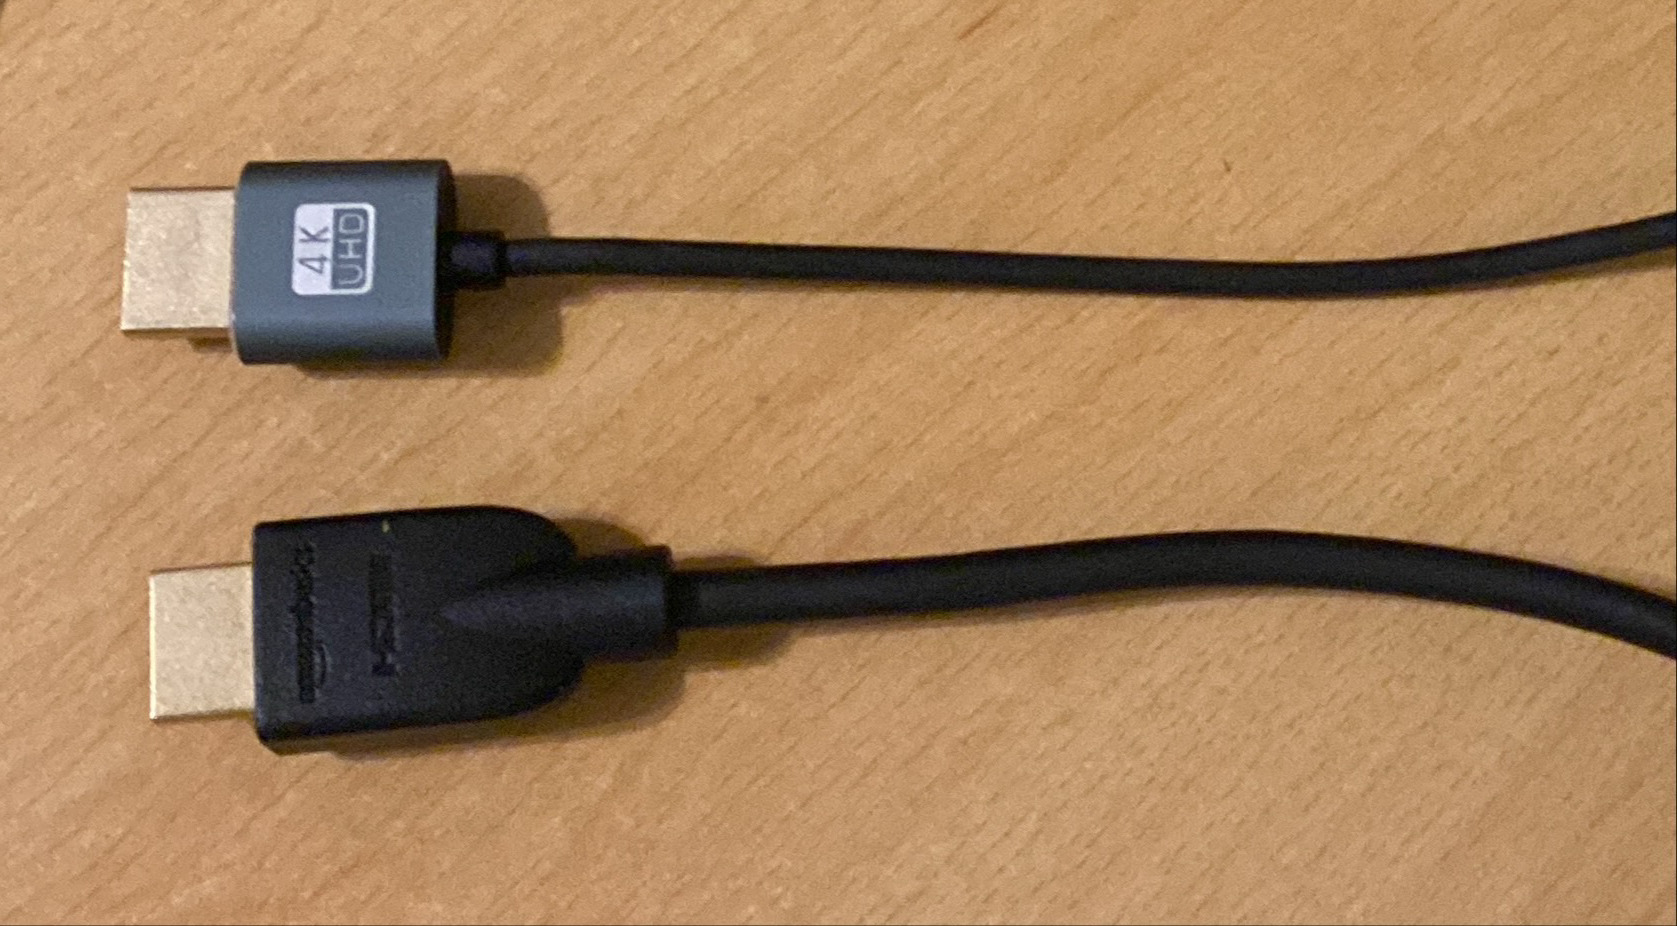
\includegraphics[width=0.7\linewidth]{images/bad-and-good-video-cables.jpg}
\end{figure}

    \subsection{Geen lampjes bij het inschakelen}
    Als de MEGA65 bij het inschakelen soms geen lampjes laat zien, heeft dit te maken met bepaalde digitale video-apparaten die op het moment dat de MEGA65 uitstaat aangesloten zijn en onvoldoende vermogen leveren om de CPLD van het toetsenbord correct van stroom te voorzien, maar wel genoeg om te voorkomen dat deze goed kan resetten wanneer de MEGA65 wordt ingeschakeld. Het verwijderen van de digitale videokabel en het opnieuw inschakelen van het apparaat lost het probleem op.

\section{Vivado}
    \subsection{RAM-vereisten}
    \begin{tcolorbox}[colback=black,coltext=white]
    \begin{lstlisting}
INFO: [Synth 8-256] done synthesizing module 'ram32x1024' [/home/....]
INFO: [Synth 8-256] synthesizing module 'charrom' [/home/....]
    /opt/Xilinx/Vivado/2019.2/bin/loader: line 280: 2317 killed
    WARNING: [Vivado 12-8222] Failed run(s) : 'synth\_1'
        ERROR: Application Exception: failed to launch run 'impl\_1' due to failures in the following run(s):
        synth\_1
        These failed run(s) need to be reset prior to launching 'impl\_1' again.
    \end{lstlisting}
    \end{tcolorbox}
Deze fout wordt veroorzaakt doordat Vivado crasht omdat het apparaat onvoldoende RAM heeft om Vivado uit te voeren.  Vivado heeft minimaal 4 GB RAM nodig om het MEGA65-doel te synthetiseren, maar 8 GB is beter.

\section{mega65\_ftp}
    \subsection{Ontbrekende bibliotheek}
    \begin{tcolorbox}[colback=black,coltext=white]
\begin{lstlisting}
/usr/bin/ld: cannot find -lncurses
collect2: error: ld returned 1 exit status
Makefile:474: recipe for target 'bin/mega65_ftp' failed
make: *** [bin/mega65_ftp] Error 1\end{lstlisting}
    \end{tcolorbox}
Deze fout treedt op wanneer de ncurses-bibliotheek op de computer ontbreekt bij het bouwen van het mega65\_ftp-programma.
Om dit probleem op te lossen, moet u deze afhankelijkheid installeren.

    \begin{tcolorbox}[colback=black,coltext=white]
\begin{lstlisting}
sudo apt-get install libncurses5-dev libncursesw5-dev\end{lstlisting}
    \end{tcolorbox}

